\chapter{Introduction}\label{chap:intro}

In the modern era of data-driven decision-making, the need for uncertainty quantification has increased across various disciplines: finance, autonomous driving, medicine... and any other high-stake application in which there is a huge error cost. Understanding and quantifying uncertainty is not merely about acknowledging the limits of predictive models, but about enhancing the reliability of decisions made based on these.\\

At its core, uncertainty quantification enables us to assess the confidence in the predictions made by models and to comprehend the potential variability in these predictions.

Formally, let us suppose we have $(X, Y)\in \R^d\times\R$ random variables from which $n$ samples $(X_i, Y_i)_{i=1}^{n}$ were obtained; and assume unknown both the $X$ and $Y$ marginal underlying probability distributions, as well as its joint distribution\footnote{Throughout this work, the distribution-free case will be considered: \textit{i.e.} no prior knowledge of the variables' underlying probability distributions is assumed and, thus, all Bayesian approaches will be disregarded.}. Given a new sample $X_{n+1}$ and a miscoverage level $\a\in\left[ 0, 1\right]$, we would like to estimate a predictive interval $\Ca$ such that the probability of $Y_{n+1}$ falling into $\Ca$ is at least $1-\a$, \textit{i.e.}

\begin{equation*}
    \P \{ Y_{n+1} \in \Ca\left(X_{n+1}\right) \} \geq 1 - \a
\end{equation*}

Note that, while retaining statistical coverage, $\Ca$ should be as small as possible to be informative. Furthermore, the intervals should be as much adaptive as possible, seeking for conditional coverage as upper limit (contrarily to non-adaptive marginal coverage). These are defined as:  
\begin{itemize}
    \item \textbf{Marginal} coverage: $\mathbb{P}\left\{Y_{n+1} \in \Hat{\Ca}\left(X_{n+1}\right)\right\}$ the errors may differ across regions of the input space (\textit{i.e.} non-adaptive)
    \item \textbf{Conditional} coverage: $\mathbb{P}\left\{Y_{n+1} \in \Hat{\Ca}\left(X_{n+1}\right) \mid X_{n+1}\right\}$ errors are evenly distributed (\textit{i.e.} fully adaptive)
\end{itemize}

Obviously, conditional coverage is stronger than marginal coverage as it allows to better represent the underlying phenomena, see Figure \ref{fig:coverage}. However, as it will be discussed in \ref{guarantees:limits}, without any distributional assumption conditional coverage cannot be guaranteed; see \cite{lei2014}; \cite{vovk2012} and \cite{barber2021a}.

\begin{figure}[ht]
    \centering
    \begin{subfigure}[b]{0.3\textwidth}
        \centering
        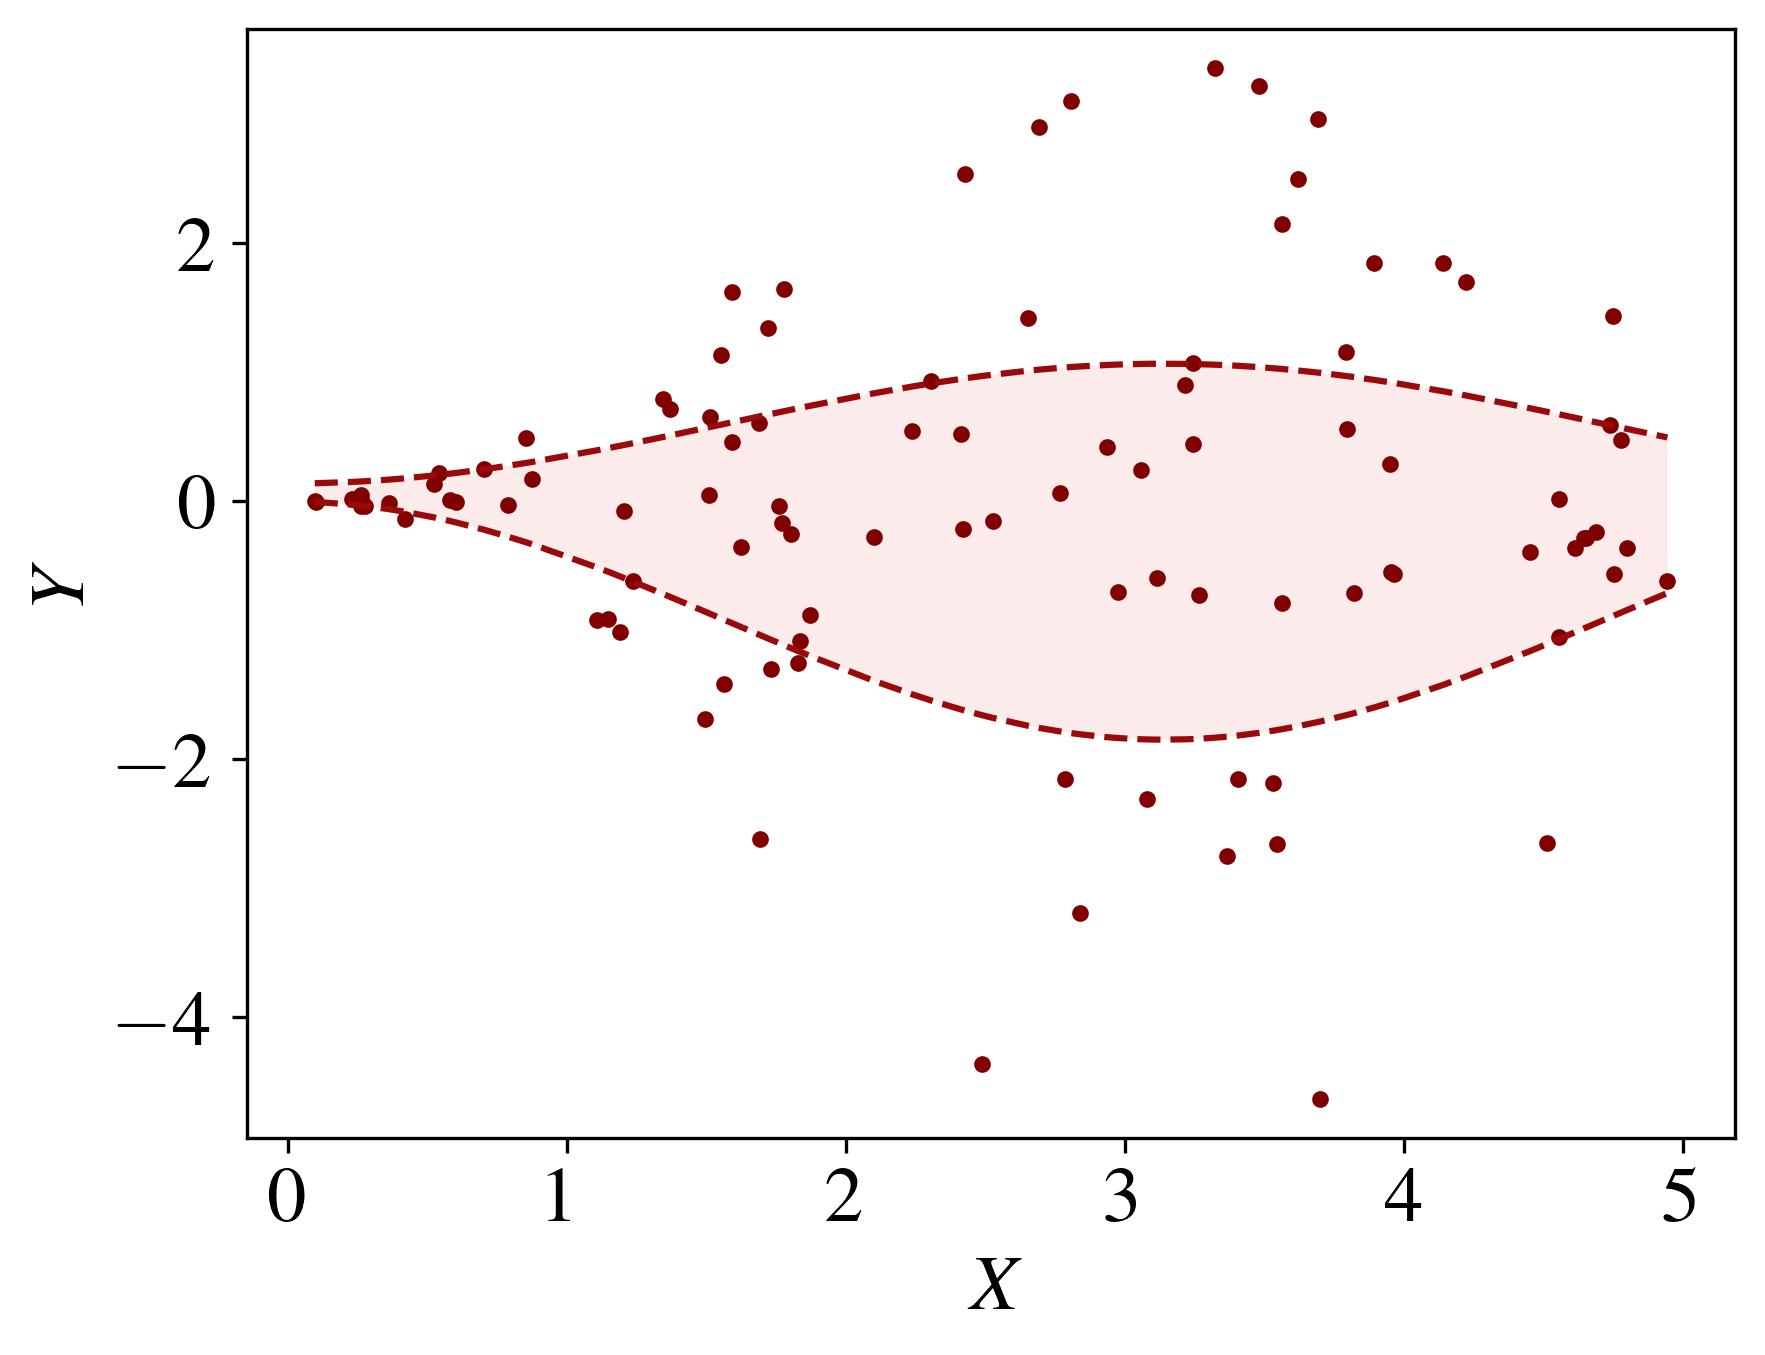
\includegraphics[width=\textwidth]{Figures/coverage/no-coverage.png}
        \caption{No coverage}
        \label{fig:coverage:no-cover}
    \end{subfigure}
    \hfill
    \begin{subfigure}[b]{0.3\textwidth}
        \centering
        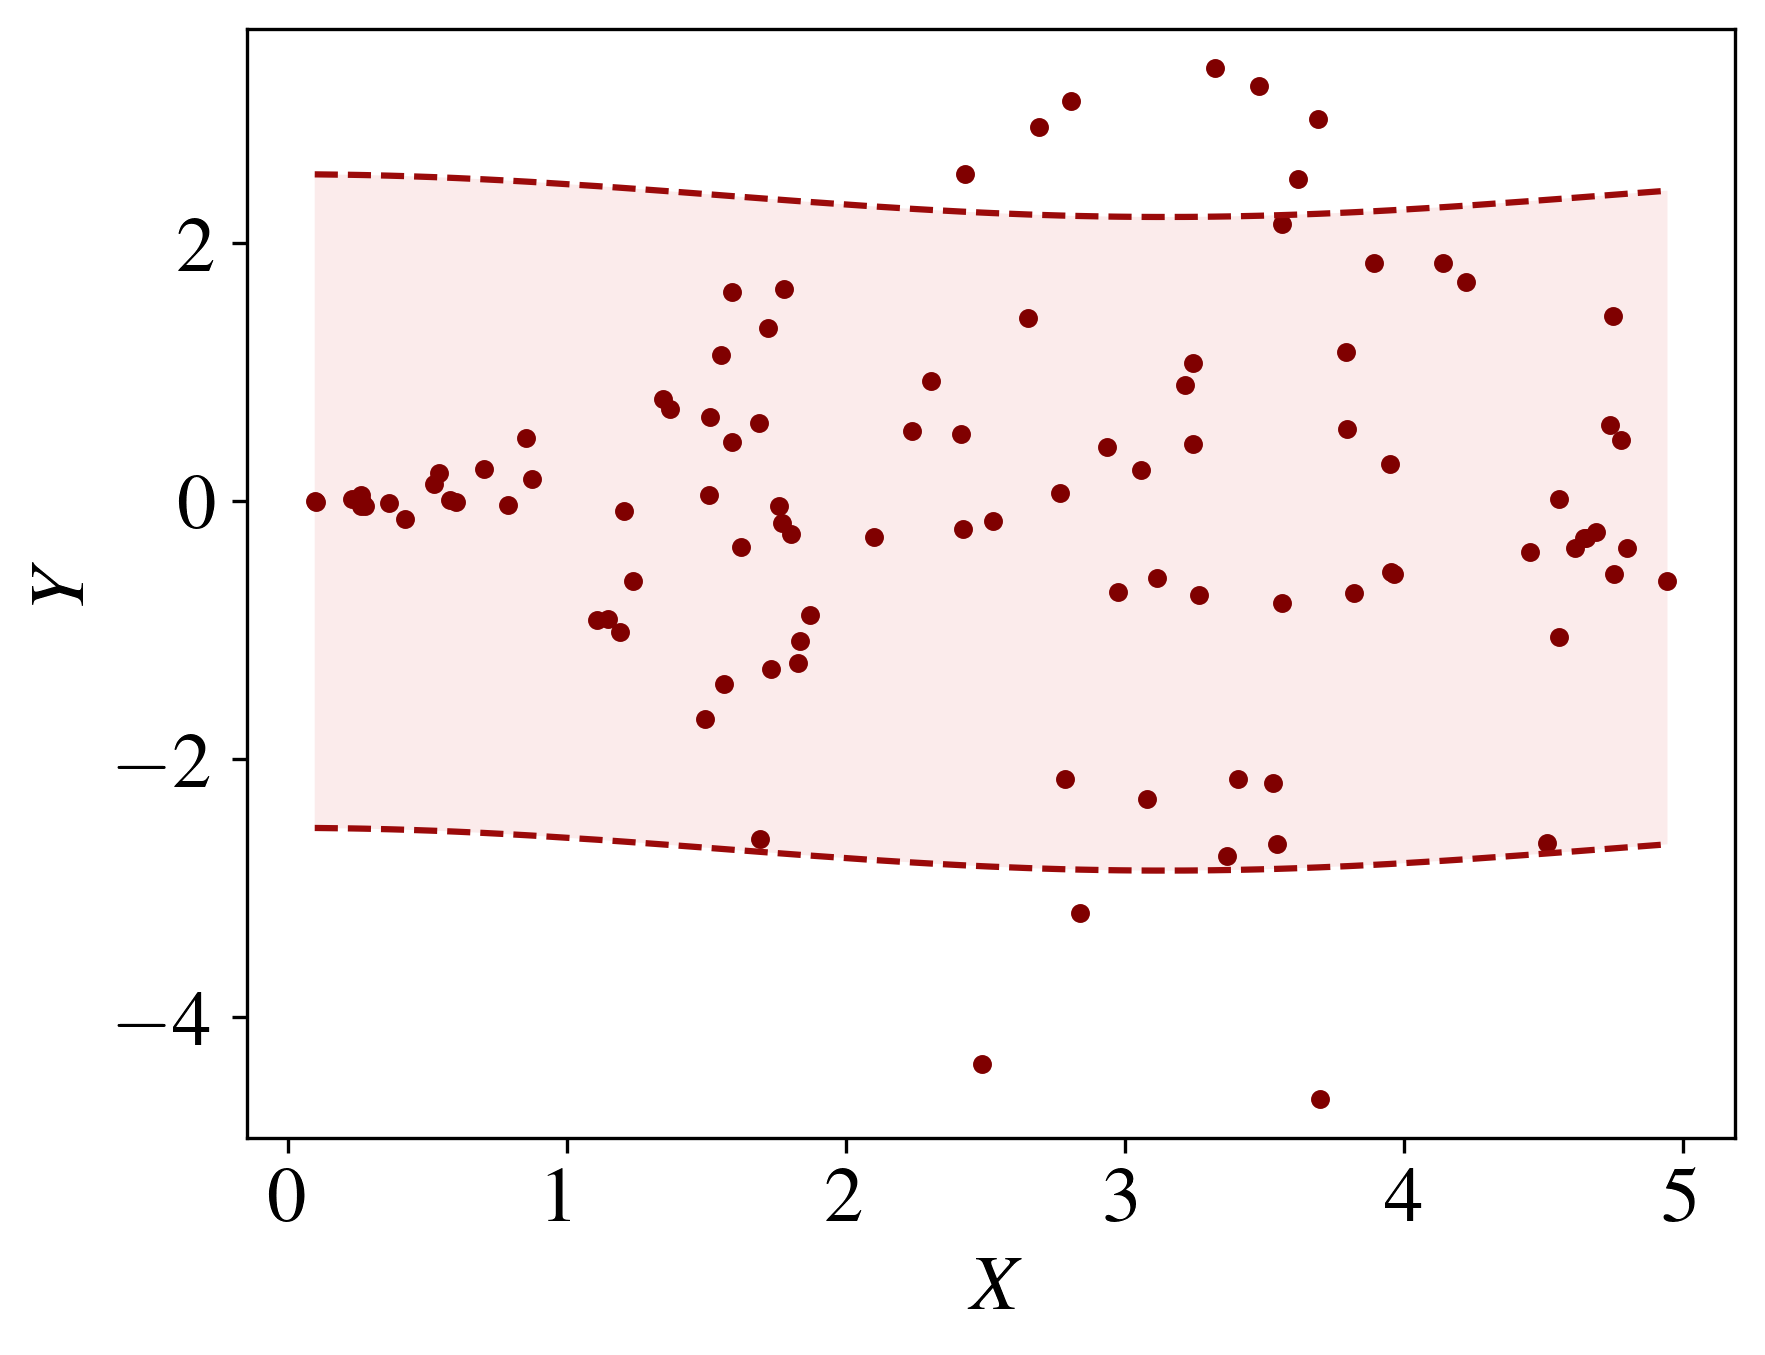
\includegraphics[width=\textwidth]{Figures/coverage/marginal-coverage.png}
        \caption{Marginal coverage}
        \label{fig:coverage:marg-cover}
    \end{subfigure}
    \hfill
    \begin{subfigure}[b]{0.3\textwidth}
        \centering
        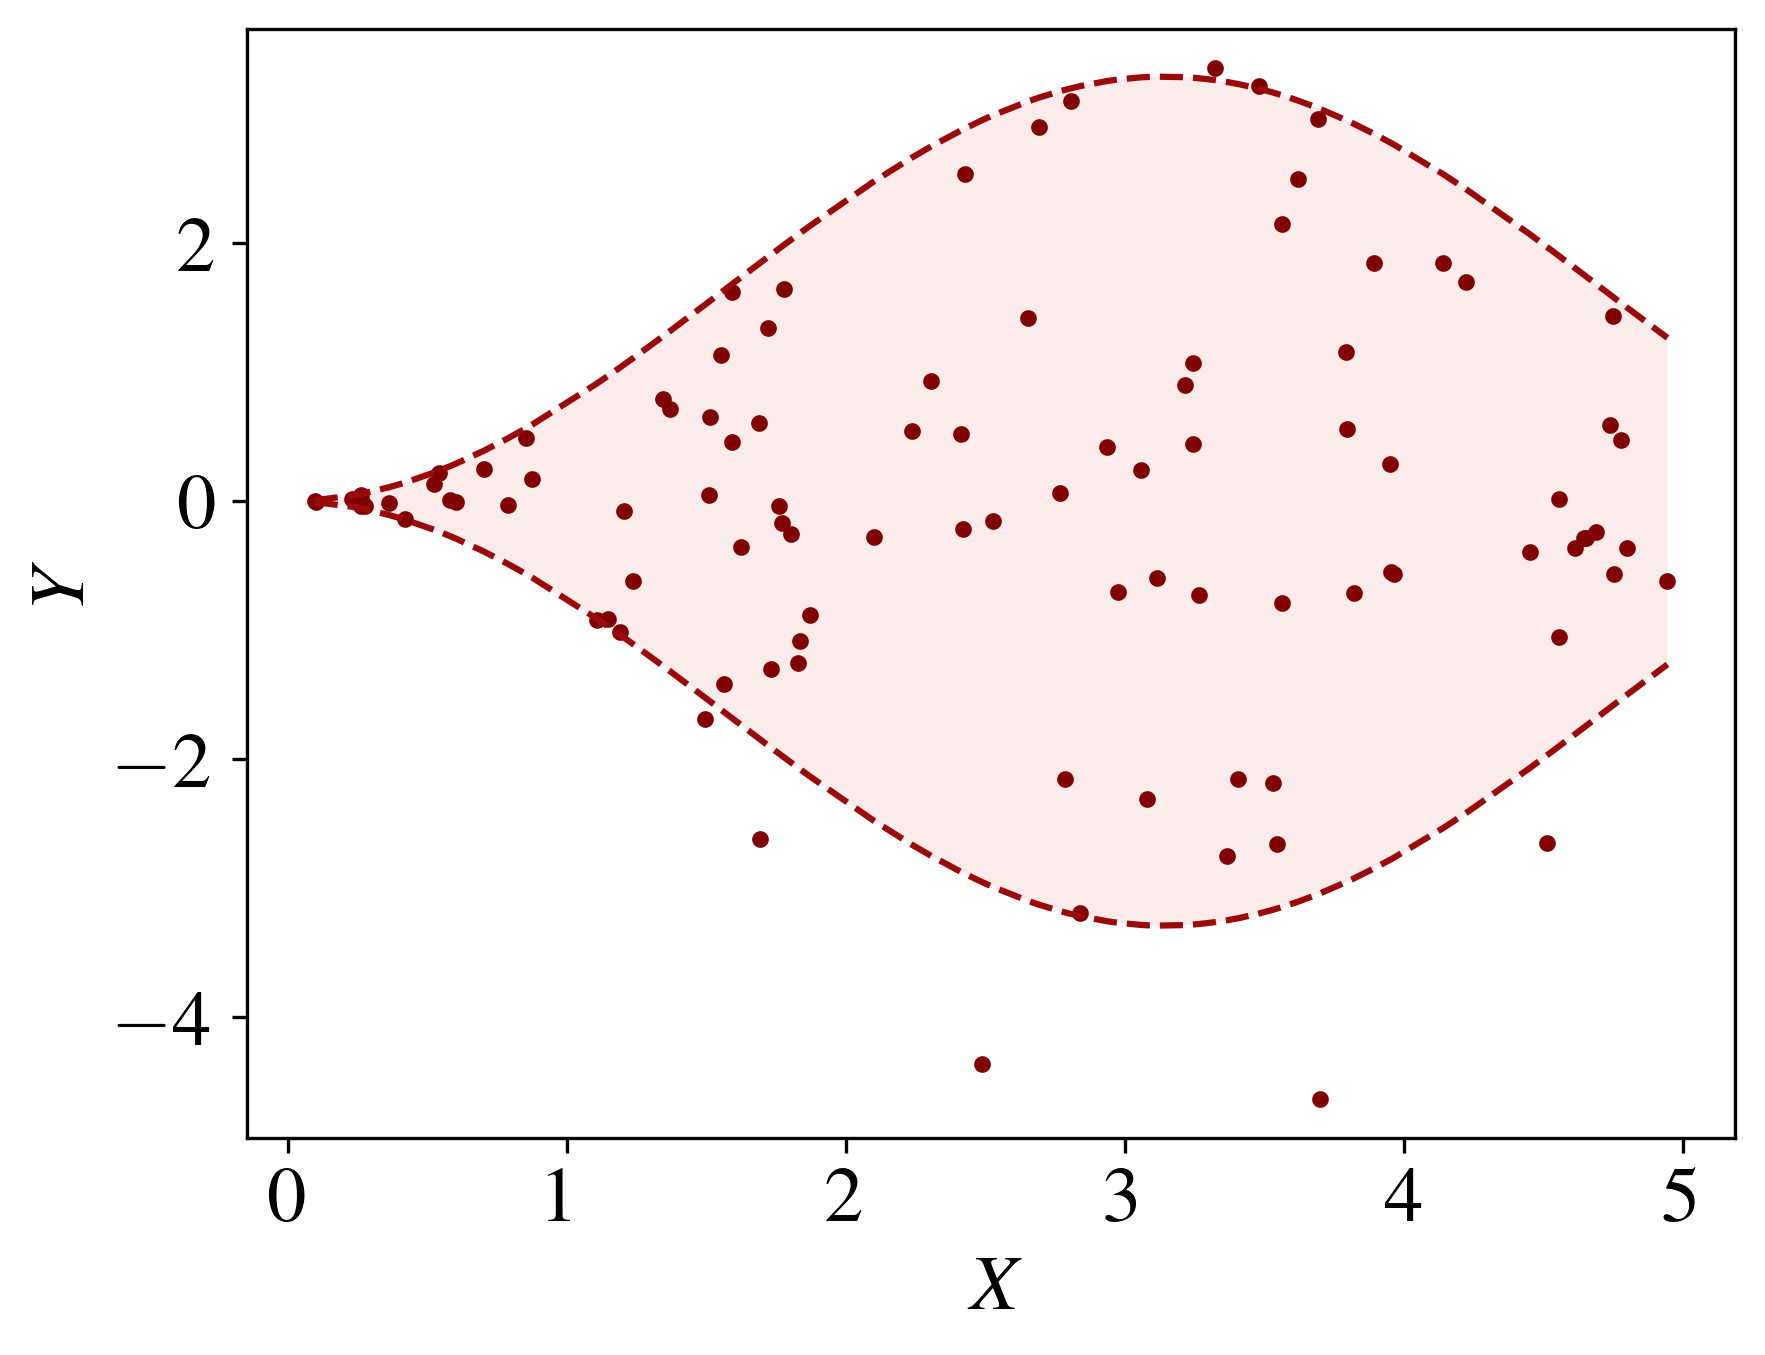
\includegraphics[width=\textwidth]{Figures/coverage/conditional-coverage.png}
        \caption{Conditional coverage}
        \label{fig:coverage:cond-cover}
    \end{subfigure}
    \caption{Different types of coverage. Plots based in \cite{cptuto}.}
    \label{fig:coverage}
\end{figure}

Now, in the general setup, these predictions intervals $\Ca$ should be valid in finite samples and agnostic not only to the data distribution but also to the model used to predict $\Hat{Y}_{n+1}$. 

Within this data-agnostic setup, in section \ref{sec:intro-quantile} quantile regression is reviewed as a historical baseline; then, in section \ref{sec:intro-conformal} conformal prediction will be presented as means of producing $\Ca$ with statistical valid coverage.

\section{Quantile regression}\label{sec:intro-quantile}

Introduced by \cite{koenker}, quantile regression focuses on estimating either boundaries of the distribution (quantiles) for a regression problem. Unlike classical linear regression, which predicts dependent variable's median given independent variables; quantile regression predicts a quantile, providing a more comprehensive analysis of possible outcome distributions.\\

Essentially, given the quantile level $\beta\in\left[0,\ 1\right]$, one can find a estimator for $\beta$ by adapting the loss function using the so-called \textit{pinball loss}:
$$ \ell_\beta\left(Y, Y^{\prime}\right)=\beta\left|Y-Y^{\prime}\right| \mathbb{1}_{\left\{\left|Y-Y^{\prime}\right| \geq 0\right\}}+(1-\beta)\left|Y-Y^{\prime}\right| \mathbb{1}_{\left\{\left|Y-Y^{\prime}\right| \leq 0\right\}} $$

Thence, during the fitting process of a estimator $\mu_\beta$ for the quantile $\beta$ - where $Y\sim \mu\left(X\right)$ -, the following loss function can be defined: $$L_{\mu_\beta}(X, Y):= \mathbb{E}\left[\ell_\beta\left(Y,\Hat{\mu_{\beta}}(X)\right)\right],$$ as the loss function.

As discussed by \cite{cptuto}, if $\Hat{\mu}\in \mathrm{argmin}_{\mu} L_{\mu_\beta}$, then $\Hat{\mu}\equiv Q_{X|Y}(\beta):=\mathrm{inf}\{x\in\R,\mathbb{P}(X\leq x|Y)\geq \beta\}$ is the $\beta$ quantile function.\\

Thus, the naive approach to obtain a predictive interval with $\alpha$ miscoverage level ($1-\a$ confidence) could be to fit the dependent variable's distribution, in terms of the independents $X$, with this adapted loss function and, then, prescribe:
$$ \Ca(X_{n+1}) = \left[ \Hat{\mu}_{\frac{\a}{2}}\left(X_{n+1}\right),\ \Hat{\mu}_{1-\frac{\a}{2}}\left(X_{n+1}\right) \right], $$ for a new sample $X_{n+1}$.

However, since $\mu_{\frac{\a}{2}}$ \& $\mu_{1-\frac{\a}{2}}$ have been trained just with $\{(X_i,Y_i)_{i=1}^n\}$, it could happen $\Ca$ is under/over-confident out of training. Namely, for a finite sample, there is no theoretical guarantee $\Ca$ has statistical valid coverage: $$ \mathbb{P}\left(Y_{n+1} \in \left[ \Hat{\mu}_{\frac{\a}{2}}\left(X_{n+1}\right),\ \Hat{\mu}_{1-\frac{\a}{2}}\left(X_{n+1}\right) \right] \right) \ne 1 - \a $$

In conclusion, though providing an approximate measure of the target's variability, quantile regression (QR) does not inherently constitute a framework for providing statistically valid predictive sets.

\section{Conformal prediction}\label{sec:intro-conformal}

Initially developed in the early 2000s by Vladimir Vovk, Alexander Gammerman, and Glenn Shafer; conformal prediction (CP) was born as a framework for producing statistically valid, data-agnostic \& distribution-free predictive sets. 

Heuristically, CP is based on the idea of using the samples data, not only to train the estimator $\mu$, but also to "conformalize" the model with the data so that the predictive sets attain the expected coverage (unlike in QR \ref{sec:intro-quantile}). 

In this sense, CP is based on the idea of using this "past" (sample) data to determine how the model errors are distributed and, thus, its conformity to the "reality". This is measured in terms of the so-called conformity score.\\ 

Notice, nevertheless, CP requires at least one assumption to ensure its validity. Since the model conformity measure is evaluated on the same samples from which the training set is created, the data needs to be \textbf{exchangeable} (\textit{i.e.} any permutation of samples should not affect the joint distribution). A thorough explanation and theoretical justification of CP, along the different methodologies to implement CP (with options for trading-off computational or statistical efficiency), is presented in chapter \ref{chap:conformal-prediction}.